% ===========================================================================
\section{Air Pollutants: An Upper Bound, and a Re-Diagnosed Blocker}
\label{sec:air}
% ===========================================================================

\subsection{The blocker was fuel analysis, not emission factors}

This sector's air-pollutant layer was previously recorded in this inventory's completeness
table as not estimated, blocked on EMEP/EEA large-combustion factors that the agency no longer
serves in a retrievable form. Working back to the primary tables showed that diagnosis was
wrong, and correcting it is a more useful result than the layer itself.

US EPA's AP-42 gives no coal \SOtwo{} factor as a fixed value. For bituminous coal,
Table~1.1-3 publishes $38S$, where $S$ is the sulfur weight percent of the coal actually
burned; for lignite---which is what \SI{79}{\percent} of this fleet's coal energy is---the
separately fetched Section~1.7 publishes $30S$ (its own footnote scales the factor $22S$ to
$34S$ with ash sodium, which is not held here, so the table's default is carried).
Table~1.3-1 publishes $157S$ for No.~6 fuel oil. Filterable particulate is $10A$
(bituminous, Table~1.1-4) and $6.5A$ (lignite, Table~1.7-4), functions of ash content.

The factors were never missing. What is missing is the \emph{fuel analysis} they scale with,
and NEPRA publishes none. That is a different problem with a different solution: no amount of
searching for factor tables would have closed it, and the earlier note would have sent a
reader looking in the wrong place.

\subsection{Fuel quality as a published range}

Published Thar lignite sulfur spans \SIrange{0.26}{2.90}{\percent}---a factor of eleven.
Ash is better constrained, with two published means at
\SI{6.42}{} and \SI{6.83}{\percent}.

Sulfur and ash are therefore carried as ranges, with the central value the geometric mean and
the uncertainty read off the range---the same treatment this inventory's fugitives sector gives
IPCC's published factor ranges, using the same function so the two cannot drift apart on the
convention. The Thar ranges belong to the lignite share by construction; the imported
bituminous burned at Sahiwal, Port Qasim and Hub has no consignment analysis in anything read
here, so the bituminous share carries the same ranges as a \emph{declared proxy}---imported
bituminous is typically lower-sulfur than this range's centre, so if anything the bituminous
side of the bound is generous, and the proxy is recorded in the fuel-quality file rather than
silently reused.

\subsection{The coal rank split, and why it raised the bound by half}

Coal was previously one stream on the bituminous section. Since the Thar-lignite split,
\SI{79}{\percent} of the coal energy (\texttt{coal\_lignite\_share}, generation-weighted
from the plant fuel ledger, $\pm$\SI{12}{\percent}) rides Section~1.7's own factors and
lignite's IPCC net calorific value of \SI{11.9}{\tera\joule\per\giga\gram}, the remainder
Section~1.1's on \SI{25.8}{}. The rank split moves the bound substantially \emph{upward}:
a tonne of lignite carries less than half the energy of a tonne of bituminous coal, so a
per-tonne factor scaled by the same sulfur or ash nearly doubles per terajoule---the same
arithmetic through which the greenhouse-gas layer's rank blend works, now applied where it
bites hardest. The firing configuration is a declared assumption (pulverized dry-bottom
tangential, the configuration whose \NOx{} factor Section~1.7 rates A); no Pakistani
document read here states the Thar boilers' firing arrangement. Lignite CO is ND in
Table~1.7-1 for this configuration and is therefore absent rather than zero-filled. Grid
bagasse cogeneration enters the layer from Section~1.8 on the same fuel energy the
greenhouse-gas layer burns---uncontrolled filterable PM and \NOx{} only, because the
section publishes no \SOtwo{} or CO factor for bagasse, whose sulfur it describes as
characteristically negligible.

\subsection{The result, labelled as what it is}

\begin{table}[htbp]
\centering
\footnotesize
\begin{tabular}{@{}lrl@{}}
\toprule
\textbf{Pollutant} & \textbf{kt/yr} & \textbf{AP-42 source} \\
\midrule
PM (filterable) & 362.3 & 1.7-4 ($6.5A$), 1.1-4 ($10A$), 1.8-1, 1.4-2 \\
\SOtwo{}        & 208.7 & 1.7-1 ($30S$), 1.1-3 ($38S$), 1.3-1 ($157S$), 1.4-2 \\
\NOx{}          & 113.4 & 1.7-1, 1.1-3, 1.3-1, 1.8-1, 1.4-1/3.1-1 \\
PM\textsubscript{10} & 118.3 & 1.7-7 ($2.3A$), 1.1-4 ($2.3A$), 1.4-2 \\
PM\textsubscript{2.5} & 34.3 & 1.7-7 ($0.66A$), 1.1-6 ($0.6A$), 1.4-2 \\
CO              &  11.9 & 1.1-3, 1.3-1, 1.4-1 \\
VOC             &   0.7 & 1.4-2 \\
\bottomrule
\end{tabular}
\caption{Grid only, FY2023--24 fuel, \textbf{uncontrolled}---an uncontrolled
screening scenario, each coal rank on its own AP-42 section since the Thar-lignite split.
Captive self-generation is IPCC 1.A.2 and is priced once, in the industrial air layer
(engine and turbine factors), so it no longer appears here.
Applied to the same terajoules
the greenhouse-gas layer burns, so both inventories describe the same combustion.}
\label{tab:air}
\end{table}

\begin{figure}[htbp]
\centering
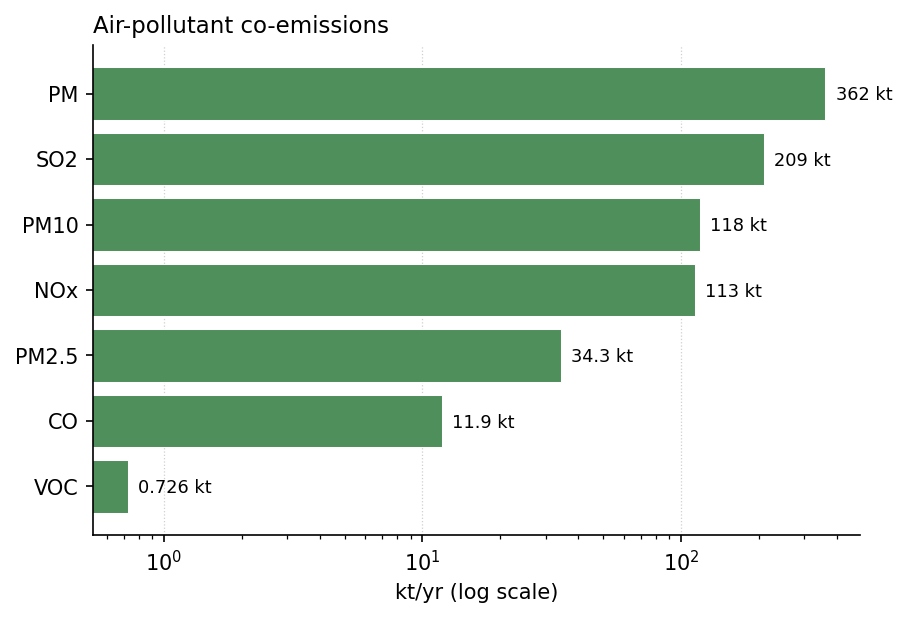
\includegraphics[width=\linewidth]{power_air.png}
\caption{The same figures on a log axis, which the range demands.}
\label{fig:air}
\end{figure}

\textbf{These are uncontrolled factors, and that word carries the whole caveat.} AP-42's
uncontrolled rows describe what leaves the furnace, not what leaves the stack. Pakistan's
supercritical coal units were built with electrostatic precipitators and the newer ones with
flue-gas desulphurisation, which remove most of the particulate and much of the sulphur. No
national dataset records which control is fitted where or how it performs.

Applying a removal efficiency would therefore mean inventing the number that matters most---it
spans an order of magnitude between uncontrolled and well-controlled. The bound is reported as
a bound, and the estimate of what the fleet actually emits is left not estimated, with the
missing parameter named. A number labelled as a bound is useful; the same number labelled as
an estimate would not be.

Where that parameter lives is now established rather than guessed. All five of NEPRA's
Licensees HSE Performance Evaluation Reports (2021 through 2024--25) were obtained and
audited for this revision: they publish no per-plant control equipment, emissions or
measurements---they are occupational-safety scorecards, one aggregate points total per
company---but their evaluation questionnaire scores licensees on ``pollution control
measures related to air quality'' and on whether an environmental monitoring report was
submitted. The controlled-emissions data this layer needs therefore exists at the
regulator as unpublished licensee submissions under the Power Safety Code, and the
concrete route to it is a request to NEPRA's HSE department, not a further search of the
published record.

\subsection{PM\texorpdfstring{\textsubscript{2.5}}{2.5} from the size distribution, with its
own check}

An earlier version of this layer carried no PM\textsubscript{2.5} row, deliberately: AP-42
Table~1.1-4 gives filterable PM and PM\textsubscript{10} for coal but no
PM\textsubscript{2.5}, and reporting the gas figure alone---about \SI{1}{\kilo\tonne},
because AP-42 notes all gas particulate is under a micron---would have read as power being
negligible for fine particulate against residential biomass at \SI{282}{\kilo\tonne} under
that sector's reference configuration, which
uncontrolled coal is not.

The missing piece was the cumulative particle-size distributions---and each rank has its
own. Table~1.1-6 (bituminous, dry-bottom pulverised) puts \SI{6}{\percent} of filterable
mass at or below \SI{2.5}{\micro\metre}: a cumulative factor of $0.6A$~lb/ton, which the
table rates C---below the A of the mass factor it scales, as a derived number should be.
The same distribution puts \SI{23}{\percent} at or below \SI{10}{\micro\metre}, $2.3A$,
exactly the PM\textsubscript{10} factor Table~1.1-4 already supplied; the two tables
reproducing each other is the check on the transcription. Lignite's own Table~1.7-7 is
coarser-shifted but sits on a heavier per-terajoule mass: \SI{10}{\percent} at
\SI{2.5}{\micro\metre} ($0.66A$) and \SI{35}{\percent} at \SI{10}{\micro\metre} ($2.3A$) of
the $6.5A$ tangential filterable factor. The result is \SI{34.32}{\kilo\tonne} of
uncontrolled PM\textsubscript{2.5}, \SI{33.31}{} of it from coal---roughly double the
pre-split figure, because lignite's tonnage per terajoule doubles the ash-scaled
mass---carried with the same
bound-not-estimate caveat as every row above---and for fine particulate that caveat bites
hardest, because electrostatic precipitators remove fine mass least efficiently exactly
where the health burden concentrates.

\subsection{A convergence that dissolved, which is the more instructive record}

The consolidated plant workbook that supplied this paper's captive register computes its own
grid \SOtwo{} for 2024, on a generation basis with kilogram-per-megawatt-hour factors, at
\SI{253.2}{\kilo\tonne}. Before the rank split, the AP-42 fuel-basis figure sat within
within a few per cent of it, and an earlier edition of this section recorded that agreement
with the warning that it was a coincidence of assumptions rather than corroboration---both
routes embedded the same all-bituminous reading of the coal fleet. The rank split proved
the warning right by dissolving the agreement: on each rank's own section and calorific
value the figure is \SI{208.7}{\kilo\tonne}, \SI{17.6}{\percent} below the workbook---it
read \SI{399.4}{\kilo\tonne} until rc60, when the oil and diesel share of this screening
narrowed to the fuel the plant-level admission register does not price, and higher again
until the coal re-base, which moved it to the other side of the workbook. That reversal is the same point made twice: this screening is coal energy times
a sulphur content, so it tracks whichever coal account is booked, while the workbook's
\SI{253.2}{\kilo\tonne} does not move at all. The agreement was never evidence and
neither is the disagreement's direction. The
divergence now \emph{measures} the shared assumption the old agreement concealed. Two
estimates that guessed the same missing parameter agreed; correcting the parameter on one
side moved it, which is exactly what agreement-by-shared-guess predicts and
corroboration does not.

\subsection{Gas \texorpdfstring{\NOx{}}{NOx}: the ledger settles the combustor question,
with a residual}

AP-42 Chapter~1.4 is an \emph{external combustion} chapter---boilers---while much of
Pakistan's gas fleet is combined-cycle, which is Chapter~3.1, and the two uncontrolled
\NOx{} factors differ: $2.7\times10^{-1}$~lb/MMBtu for a large wall-fired boiler against
$3.2\times10^{-1}$ for a gas turbine, both rated A. An earlier version of this layer called
gas \NOx{} its weakest row because NEPRA's national fuel table reports fuel without plant
type. The plant ledger changes that: it carries heat rates, and a plant at or below
\SI{9000}{\kilo\joule\per\kilo\watt\hour} net---\SI{40}{\percent} efficiency---can
physically only be a combined cycle. Heat rate is trusted over names, because names lie
here: Bin Qasim TPS-II and TPS-III are combined-cycle blocks behind steam-era names, and
Guddu's units 14--16 carry a heat rate no combined cycle designs to. Names decide only where
they assert turbine hardware (GTPS, CCPP), which heat rate cannot separate from a steam
plant at simple-cycle efficiencies.

On FY2023--24 energy the grid gas fleet classifies as \SI{80.2}{\percent} turbine,
\SI{13.7}{\percent} boiler, and \SI{6.1}{\percent} unresolved---three plants in the
9{,}000--10{,}500 band, where a degraded combined cycle and a steam plant are
indistinguishable from the ledger. The grid gas \NOx{} factor is the energy-weighted blend,
with the unresolved share kept on the boiler factor and reported here rather than assigned.
Because the turbine factor is the higher one, resolving the fleet \emph{raises} gas \NOx{}
by about \SI{13}{\percent} over the all-boiler assumption; the total above moves
accordingly. Only \NOx{} is split: the CO factors of the two chapters are numerically
indistinguishable, and sulphur passes through to \SOtwo{} regardless of how the gas is
burned. Captive self-generation has left this table: IPCC 2006 books autoproducer generation
under 1.A.2, and the industrial air layer prices it on stationary-engine and gas-turbine factors
under declared fleet shares, reported once under industry.
